\documentclass[11pt,a4paper]{article}
\usepackage[T1]{fontenc}
\usepackage{lmodern}
\usepackage[margin=2.3cm]{geometry}
\usepackage{amsmath,amssymb}
\usepackage{graphicx}
\usepackage{booktabs}
\usepackage{placeins}
\usepackage{microtype}
\usepackage{enumitem}
\usepackage[font=small,labelfont=bf]{caption}
\usepackage[dvipsnames]{xcolor}
\usepackage[most]{tcolorbox}
\usepackage[colorlinks=true,linkcolor=MidnightBlue,urlcolor=MidnightBlue]{hyperref}

\graphicspath{{../../lsb/figs/}}
\setlist{itemsep=2pt,topsep=4pt}
\newcommand{\CL}{C_L}
\newcommand{\af}{\alpha_f}
\newcommand{\ate}{\alpha_{TE}}

\newtcolorbox{definitionbox}{colback=Goldenrod!12,colframe=BrickRed,boxrule=1.2pt,
  arc=2pt,left=6pt,right=6pt,top=4pt,bottom=4pt,
  title={\bfseries\large What ``trailing-edge separation'' ($\ate$) means in this report},
  coltitle=white,colbacktitle=BrickRed}

\title{Does the laminar separation bubble set the cubic?\\[2pt]
\large Tests of the LSB hypothesis on the thick flat plate ($t/c = 0.023$), Re = 500 (steady)}
\author{LSB hypothesis report}
\date{9 October 2026}

\begin{document}
\maketitle

\begin{definitionbox}
In this report, \textbf{``trailing-edge separation'' means the angle at which the
leading-edge bubble's reattachment point reaches the trailing edge}:
\[
  \ate = 8.40^\circ, \qquad \text{bracketed in } (8.3^\circ,\ 8.4^\circ].
\]
This definition was \emph{chosen} for the plate (decision of 9 October 2026). It is
\textbf{not} the usual meaning of the term:
\begin{itemize}[leftmargin=*]
\item \textbf{The plate's trailing edge never separates on its own.} Below $\af$ the upper
  surface is attached all the way to the trailing edge. No separation starts at the trailing
  edge and moves forward.
\item \textbf{The bubble does not burst or open into the wake} anywhere in the computed range
  (up to $9.0^\circ$). Above $8.4^\circ$ it covers the whole upper surface but stays closed. Its
  rear stagnation point is pinned in the corner where the flat surface meets the rounded trailing
  edge ($x_{\text{flat}} = 0.9892c$). There is no reversed flow in the near wake.
\item \textbf{The value $8.40^\circ$ is an extrapolation.} Between $8.0^\circ$ and $8.3^\circ$ the
  reattachment point moves downstream linearly, at $1.466c$ per degree. That line reaches
  $x_{\text{flat}}$ at $8.405^\circ$. Above it, reattachment only creeps into the corner:
  $0.967, 0.979, 0.983, 0.985, 0.987, 0.988, 0.989$ from $8.4^\circ$ to $9.0^\circ$.
\end{itemize}
A different definition would move $\ate$. Reversed flow in the near wake, for example, has not
happened by $9.0^\circ$, and the plate starts shedding at about $11.3^\circ$. A change of
definition would also change fits~(A) and~(B) below.
\end{definitionbox}

\section{The hypothesis and the verdict}

The hypothesis (\texttt{instructions/lsb\_hypothesis.md}) tries to explain why the cubic term
dominates less and less as the section goes from NACA0012 to NACA0006 to the plate. It attributes
this to the formation of a laminar separation bubble (LSB) and to the bubble saturating. It makes
three falsifiable claims. Here they are tested on the plate, which is the section that has a
leading-edge bubble at Re = 500.

\begin{center}
\begin{tabular}{p{0.37\linewidth}p{0.57\linewidth}}
\toprule
Claim & Verdict on the plate \\
\midrule
1. Lift is mostly linear before the LSB forms. &
\textbf{False.} Lift curves from the smallest angles. A straight line misses by 0.4\,\% on
$0$--$3^\circ$, 2.6\,\% on $0$--$6^\circ$ and 6.3\,\% on $0$--$7.75^\circ$. All of these
ranges are below $\af$, where there is no separation anywhere. \\[3pt]
2. Once the LSB forms, cubic terms explain the curvature well. &
\textbf{Not supported.} Every measure of how cubic-like the curve is changes smoothly through
$\af$. Inside $[\af,\ate]$ the local curvature, $-0.0182$ per deg$^2$, is twice what the best
two-term ($\theta$, $\theta^3$) fit implies there ($-0.0094$ per deg$^2$). \\[3pt]
3. Once ``trailing-edge separation'' happens\textsuperscript{$\dagger$}, the cubic loses
dominance. &
\textbf{Partly.} Beyond $\ate$ the slope keeps falling to the lift peak ($\CL = 0.628$ near
$10.5^\circ$), and the odd series needs $c_7$ and $c_9$. But this sets in gradually from about
$9.5^\circ$. Nothing changes at $\ate$ itself. \\
\bottomrule
\end{tabular}

\smallskip
{\small $^\dagger$ ``Trailing-edge separation'' as defined in the box above.}
\end{center}

\paragraph{What the bubble does to the lift curve.}
\begin{itemize}[leftmargin=*]
\item \textbf{There is no kink in $\CL$ at either marker.} On the fine mesh, at $0.1^\circ$
  spacing, the lift slope falls on a straight line through both (Fig.~\ref{fig:kink}).
\item \textbf{The curvature responds only slightly.} It steepens by about $5\times10^{-4}$ per
  deg$^2$ at $\af$ and stops growing after $\ate$. Both changes are the size of the force noise.
\item \textbf{The one clear sign is in the fourth difference of $\CL$} on the $0.25^\circ$
  grid. It rises from about $10^{-6}$ below $7^\circ$ to $1.8\times10^{-5}$ at
  $7.75$--$8^\circ$. Equivalently, $c_9$ grows from noise level to $1.2\times10^{-4}$ in the
  windows that reach $\af$.
\end{itemize}

\begin{figure}[h]
\centering
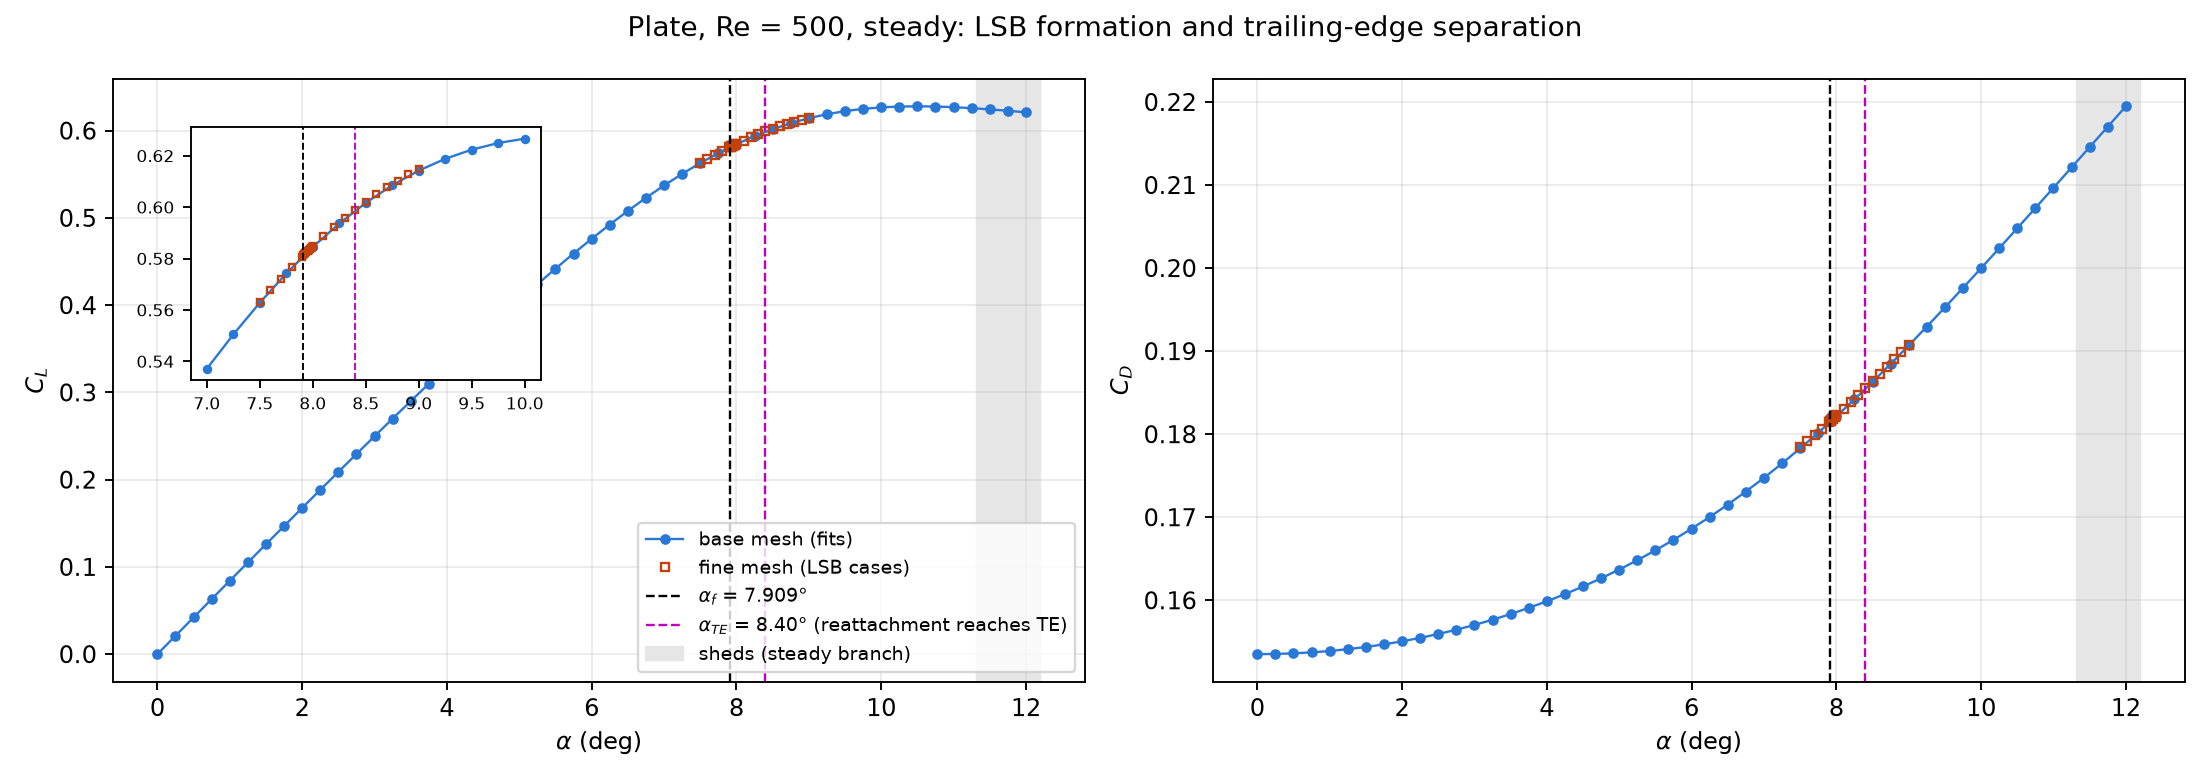
\includegraphics[width=\linewidth]{hypothesis/lift_drag_markers.png}
\caption{Lift and drag on the production mesh (blue, every $0.25^\circ$) and the fine mesh
(orange squares). Dashed lines: $\af = 7.909^\circ$ (black) and
$\ate = 8.40^\circ$ (magenta, where reattachment reaches the trailing edge, as defined above).
Grey: the flow actually sheds there, and the steady branch is shown.}
\label{fig:lift}
\end{figure}

\section{Data and markers}

\begin{itemize}[leftmargin=*]
\item \textbf{Plate geometry:} thickness $t/c = 0.023$ (2.3\,\% of chord). The section is a
  stadium: a flat plate with semicircular leading and trailing edges of radius $0.0115c$, overall
  length $c = 1$ (after the Eldredge \& Wang plate).
\item \textbf{Lift curve:} steady SIMPLE on the production plate mesh (63k cells), every
  $0.25^\circ$ from $0^\circ$ to $12^\circ$. All 49 angles pass the sweep's force-trace
  convergence test.
\item \textbf{Three machines:} the $0.25^\circ$ points were shared between OpenFOAM-dev,
  OpenFOAM~13 and OpenFOAM~v14. The second differences show no step between versions, and the
  fourth differences stay within $\pm6\times10^{-6}$. That bounds any offset between versions at
  about $4\times10^{-7}$ in $\CL$.
\item \textbf{Markers and fit~(B):} the fine mesh (91k cells, first cell $0.025/\sqrt{Re}$),
  every $0.1^\circ$ over $7.5$--$9.0^\circ$ and every $0.01^\circ$ over $7.90$--$8.00^\circ$. On
  the forces the two meshes agree to better than 0.1\,\%.
\item \textbf{Markers:}
  \begin{itemize}
  \item $\af = 7.9087^\circ$, where the smallest upper-surface $C_f$ crosses zero. It falls exactly
    linearly with angle: $C_{f,\min} = -0.00752(\alpha-7.9087)$, maximum residual
    $1.2\times10^{-6}$. On the production mesh, $\af = 7.892^\circ$.
  \item $\ate = 8.40^\circ$, as defined in the box.
  \item The plate starts shedding at about $11.33^\circ$.
  \end{itemize}
\end{itemize}

\section{Claim 1: a straight line before the bubble?}

For windows $0$--$A$ entirely below $\af$, Table~\ref{tab:c1} compares a straight line ($P_1$)
with the two-term odd fit ($P_1+P_3$). Here the cubic coefficient is expressed as $a_3$ in
$\CL = a_1\theta + a_3\theta^3$.

\begin{table}[h]
\centering\small
\begin{tabular}{lrrrrr}
\toprule
window & $\CL$ at end & max straight-line error & \% of $\CL$ & max $P_1{+}P_3$ error & $a_3$ (rad$^{-3}$) \\
\midrule
$0$--$1^\circ$ & 0.0841 & $2.6\times10^{-5}$ & 0.03 & $3.2\times10^{-7}$ & $-18.9$ \\
$0$--$2^\circ$ & 0.1676 & $2.7\times10^{-4}$ & 0.16 & $1.4\times10^{-6}$ & $-19.5$ \\
$0$--$3^\circ$ & 0.2497 & $1.0\times10^{-3}$ & 0.42 & $1.6\times10^{-5}$ & $-20.4$ \\
$0$--$4^\circ$ & 0.3296 & $2.8\times10^{-3}$ & 0.84 & $8.6\times10^{-5}$ & $-21.8$ \\
$0$--$5^\circ$ & 0.4057 & $6.2\times10^{-3}$ & 1.52 & $3.2\times10^{-4}$ & $-23.7$ \\
$0$--$6^\circ$ & 0.4760 & $1.2\times10^{-2}$ & 2.59 & $9.7\times10^{-4}$ & $-26.4$ \\
$0$--$7^\circ$ & 0.5371 & $2.3\times10^{-2}$ & 4.33 & $2.5\times10^{-3}$ & $-30.1$ \\
$0$--$7.75^\circ$ & 0.5742 & $3.6\times10^{-2}$ & 6.28 & $4.5\times10^{-3}$ & $-33.5$ \\
\bottomrule
\end{tabular}
\caption{The plate's lift is cubic from the start: $a_3 \to -18.9$ rad$^{-3}$ on the smallest
window, with no bubble and no separation anywhere.}
\label{tab:c1}
\end{table}

\begin{itemize}[leftmargin=*]
\item \textbf{``Mostly linear'' holds only up to about $2$--$3^\circ$.}
\item \textbf{By $6^\circ$ the cubic term is clearly needed:} the straight line misses by
  2.6\,\%, against 0.2\,\% for the two-term fit.
\item \textbf{This bending comes from the attached laminar boundary layer at Re = 500, not from
  the bubble.}
\end{itemize}

\section{(C) Odd Legendre fits on $0$ to $6$--$8^\circ$}

The angle is mapped to $x = \alpha/A$ and mirrored onto $[-1,1]$, and the fit uses
$P_1,P_3,P_5,P_7,P_9$ with no constant term. This is the same method as the earlier plate
Legendre fits. Each window uses every $0.25^\circ$ point it contains. The last two columns are
the two-term ($P_1+P_3$) fit rewritten in powers of $\theta$.

\begin{table}[h]
\centering\footnotesize
\setlength{\tabcolsep}{4pt}
\begin{tabular}{rrrrrrrrrrr}
\toprule
$A$ ($^\circ$) & $n$ & $c_1$ & $c_3$ & $c_5$ & $c_7$ & $c_9$ & $c_3/c_1$ & $c_5/c_3$ & $a_1$ & $a_3$ \\
\midrule
6.00 & 24 & 0.48921 & $-0.01196$ & $-0.001120$ & $-8.32\mathrm{e}{-5}$ & $-1.26\mathrm{e}{-6}$ & $-0.0244$ & 0.094 & 4.845 & $-26.40$ \\
6.25 & 25 & 0.50781 & $-0.01393$ & $-0.001421$ & $-1.11\mathrm{e}{-4}$ & $-3.77\mathrm{e}{-7}$ & $-0.0274$ & 0.102 & 4.849 & $-27.22$ \\
6.50 & 26 & 0.52612 & $-0.01617$ & $-0.001788$ & $-1.44\mathrm{e}{-4}$ & $1.62\mathrm{e}{-6}$ & $-0.0307$ & 0.111 & 4.854 & $-28.11$ \\
6.75 & 27 & 0.54410 & $-0.01871$ & $-0.002231$ & $-1.84\mathrm{e}{-4}$ & $4.92\mathrm{e}{-6}$ & $-0.0344$ & 0.119 & 4.859 & $-29.06$ \\
7.00 & 28 & 0.56172 & $-0.02159$ & $-0.002761$ & $-2.30\mathrm{e}{-4}$ & $1.11\mathrm{e}{-5}$ & $-0.0384$ & 0.128 & 4.866 & $-30.08$ \\
7.25 & 29 & 0.57894 & $-0.02484$ & $-0.003389$ & $-2.80\mathrm{e}{-4}$ & $2.26\mathrm{e}{-5}$ & $-0.0429$ & 0.136 & 4.873 & $-31.17$ \\
7.50 & 30 & 0.59574 & $-0.02850$ & $-0.004122$ & $-3.30\mathrm{e}{-4}$ & $4.20\mathrm{e}{-5}$ & $-0.0478$ & 0.145 & 4.882 & $-32.31$ \\
7.75 & 31 & 0.61207 & $-0.03260$ & $-0.004966$ & $-3.75\mathrm{e}{-4}$ & $7.23\mathrm{e}{-5}$ & $-0.0533$ & 0.152 & 4.891 & $-33.51$ \\
8.00 & 32 & 0.62789 & $-0.03719$ & $-0.005926$ & $-4.05\mathrm{e}{-4}$ & $1.17\mathrm{e}{-4}$ & $-0.0592$ & 0.159 & 4.901 & $-34.75$ \\
\bottomrule
\end{tabular}
\caption{Odd Legendre coefficients on $0$--$A$. $a_1$ is in rad$^{-1}$ and $a_3$ in rad$^{-3}$.
The two-term fit's maximum error grows from $9.7\times10^{-4}$ (0--6$^\circ$) to
$5.3\times10^{-3}$ (0--8$^\circ$).}
\label{tab:C}
\end{table}

\begin{itemize}[leftmargin=*]
\item \textbf{$c_5$ is 9--16\,\% of $c_3$ throughout}, and its share grows steadily.
\item \textbf{$a_3$ depends on the window}, drifting from $-26.4$ to $-34.8$ rad$^{-3}$. There
  is no change of trend at the windows that reach $\af$.
\item \textbf{Only $c_9$ responds near the bubble.} It is at noise level up to $6.5^\circ$, then
  grows a hundredfold.
\end{itemize}

\begin{figure}[h]
\centering
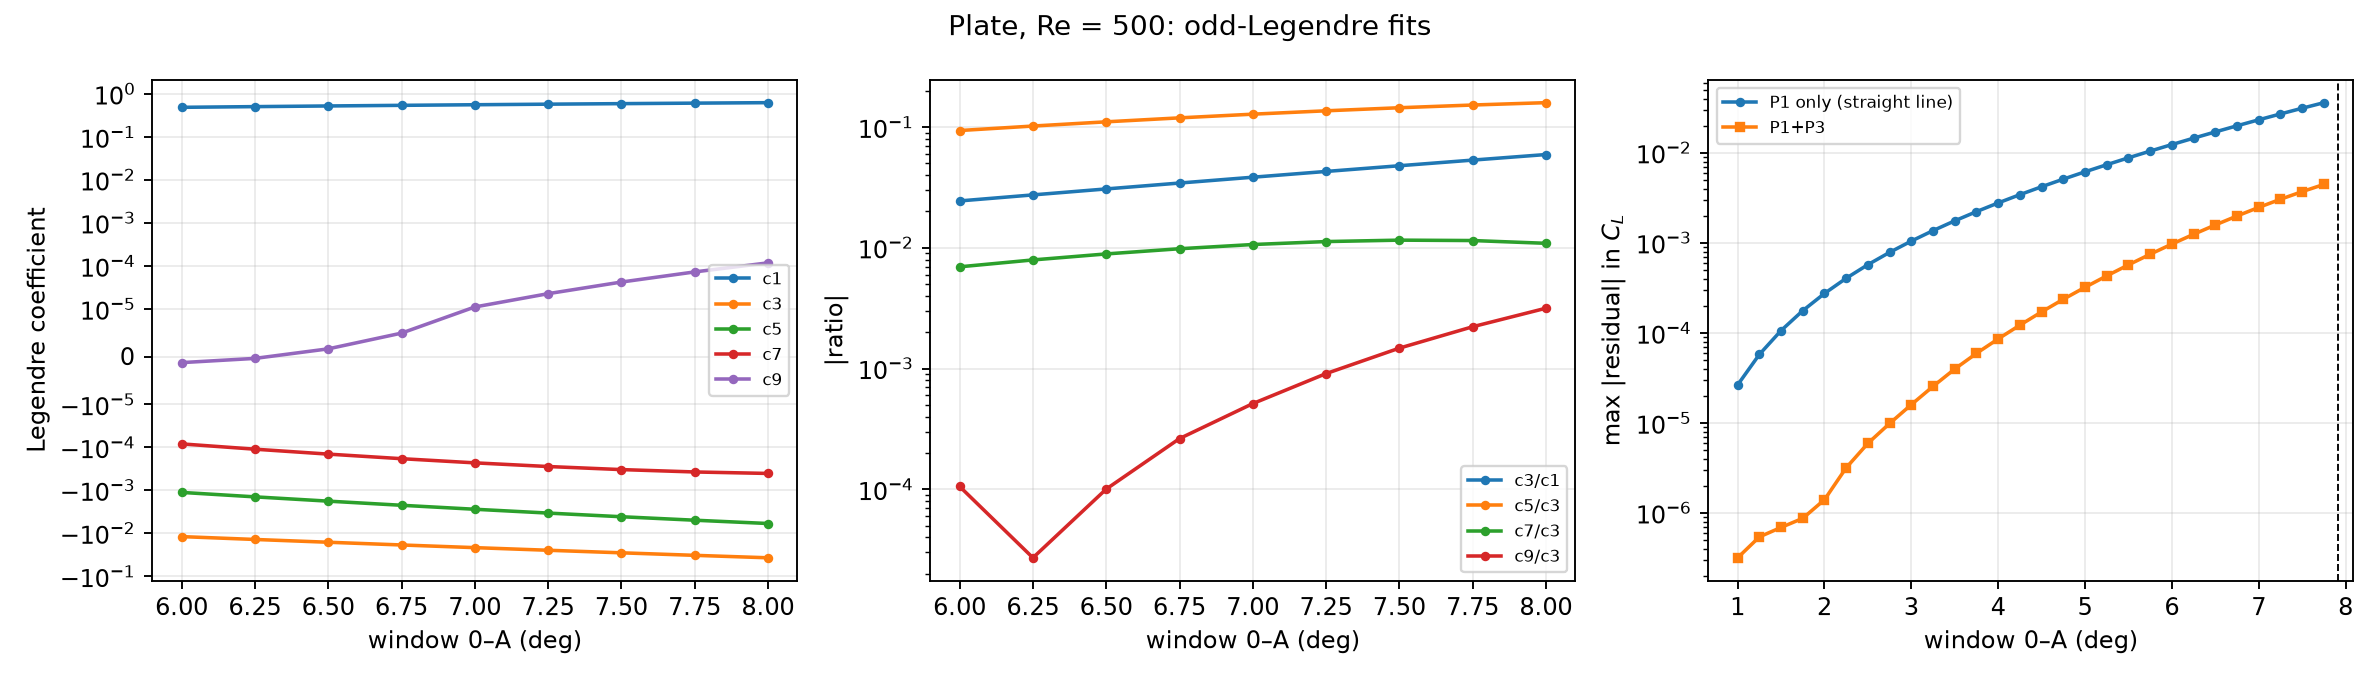
\includegraphics[width=\linewidth]{hypothesis/odd_window_scan.png}
\caption{Left: the coefficients. Centre: their ratios. Right: the largest error of a straight
line and of $P_1+P_3$ on windows $0$--$A$ below $\af$ (claim~1).}
\end{figure}

\FloatBarrier
\section{(B) Between the markers, $\af \le \alpha \le \ate$}

On the fine mesh there are 14 angles in $[7.909^\circ, 8.40^\circ]$. Mapped onto $[-1,1]$, they
are fitted to within their own noise by a parabola. Every degree, odd and even, is allowed.

\begin{center}\small
\begin{tabular}{rrrrrrr}
\toprule
degree & $c_0$ & $c_1$ & $c_2$ & $c_3$ & RMSE & max error \\
\midrule
1 & 0.590382 & 0.009031 & & & $1.6\times10^{-4}$ & $3.3\times10^{-4}$ \\
\textbf{2} & 0.590486 & 0.008960 & $-0.000366$ & & $6.7\times10^{-7}$ & $1.3\times10^{-6}$ \\
3 & 0.590487 & 0.008961 & $-0.000366$ & $-0.000002$ & $1.0\times10^{-7}$ & $1.9\times10^{-7}$ \\
\bottomrule
\end{tabular}
\end{center}

\begin{itemize}[leftmargin=*]
\item \textbf{Slope: $0.0368$ per degree $=$ \textbf{2.11 per rad}}. The curvature is $-0.0182$ per
  deg$^2$.
\item \textbf{Compared with the global two-term fit on $0$--$8.25^\circ$} ($a_1 = 4.913$,
  $a_3 = -36.0$): at mid-window that fit implies 2.72 per rad and $-0.0094$ per deg$^2$. So the
  real curve is about 23\,\% less steep and bends about twice as hard.
\item \textbf{In the bubble range, a $\theta+\theta^3$ law does not capture the curvature.}
  That is evidence against claim~2.
\end{itemize}

\section{(A) Beyond $\ate$: the slope after ``trailing-edge separation''}

\noindent\colorbox{Goldenrod!20}{\parbox{\dimexpr\linewidth-2\fboxsep}{\small
$\ate = 8.40^\circ$ here is the angle where reattachment reaches the trailing edge (see the box
on page~1). It is not a separation that starts at the trailing edge.}}

\smallskip
These fits use the production mesh, every $0.25^\circ$, mapped onto $[-1,1]$.

\begin{center}\footnotesize
\setlength{\tabcolsep}{4pt}
\begin{tabular}{lrrrr}
\toprule
fit & linear slope & mid-window slope & curvature & max error \\
\midrule
$8.5$--$12^\circ$, deg.~1 & \textbf{0.261 /rad} (0.0046 /deg) & & & $1.2\times10^{-2}$ \\
$8.5$--$12^\circ$, deg.~2 & 0.261 /rad & 0.261 /rad & $-0.0106$ /deg$^2$ & $1.7\times10^{-3}$ \\
$8.5$--$12^\circ$, deg.~3 & 0.261 /rad & 0.142 /rad & $-0.0106$ /deg$^2$ & $3.7\times10^{-5}$ \\
$8.5$--$11.25^\circ$ (no shedding), deg.~2 & \textbf{0.470 /rad} (0.0082 /deg) & 0.470 /rad & $-0.0129$ /deg$^2$ & $7.9\times10^{-4}$ \\
\bottomrule
\end{tabular}
\end{center}

\begin{itemize}[leftmargin=*]
\item \textbf{The slope after ``trailing-edge separation'' is 0.26 per rad on $8.5$--$12^\circ$}, or
  0.47 per rad if the angles that actually shed are left out.
\item \textbf{For comparison:} 2.1 per rad between the markers and 4.83 per rad at small angles.
\item \textbf{These are averages.} The pointwise slope falls continuously, from 1.83 per rad at
  $8.4^\circ$ to 1.25 per rad at $8.95^\circ$.
\item \textbf{Beyond $\ate$ the curve is shaped by its maximum} ($\CL = 0.6279$ at $10.5^\circ$).
  The local fit is dominated by the quadratic term. A purely odd series centred at $0^\circ$ can
  follow this only with growing $c_7$ and $c_9$ (Fig.~\ref{fig:dom}).
\end{itemize}

\begin{figure}[h]
\centering
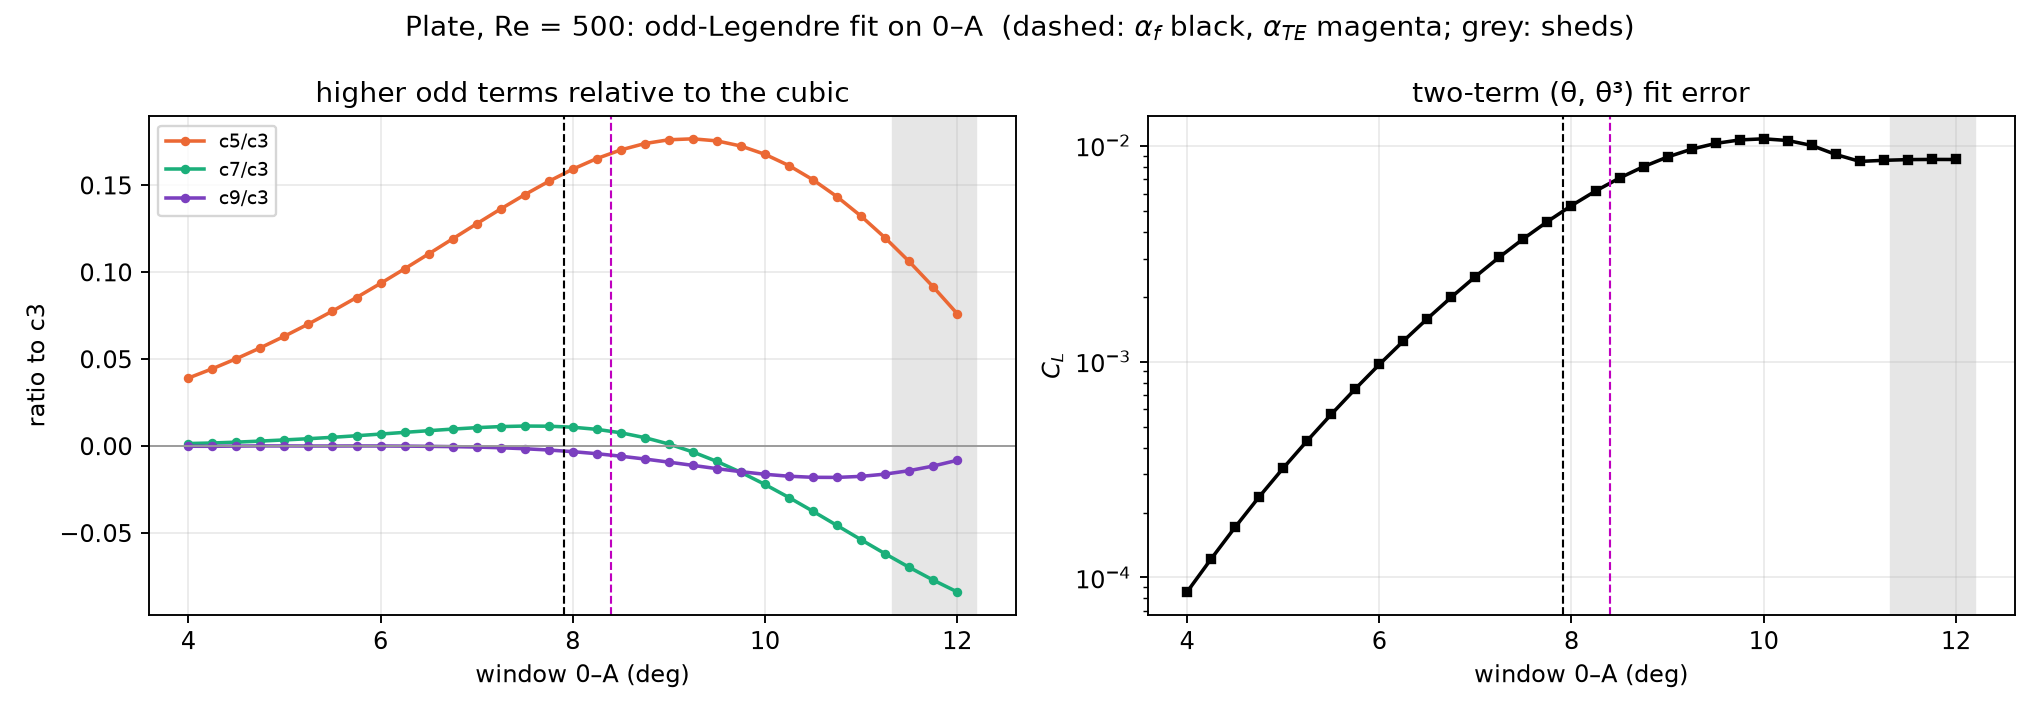
\includegraphics[width=\linewidth]{hypothesis/cubic_dominance_0to12.png}
\caption{Odd fit on $0$--$A$ for $A$ up to $12^\circ$. $c_7/c_3$ changes sign at about $9^\circ$
and grows to $-0.08$. The two-term error levels off at about $10^{-2}$. These changes are
gradual and come after $\ate$, not at it.}
\label{fig:dom}
\end{figure}

\begin{figure}[h]
\centering
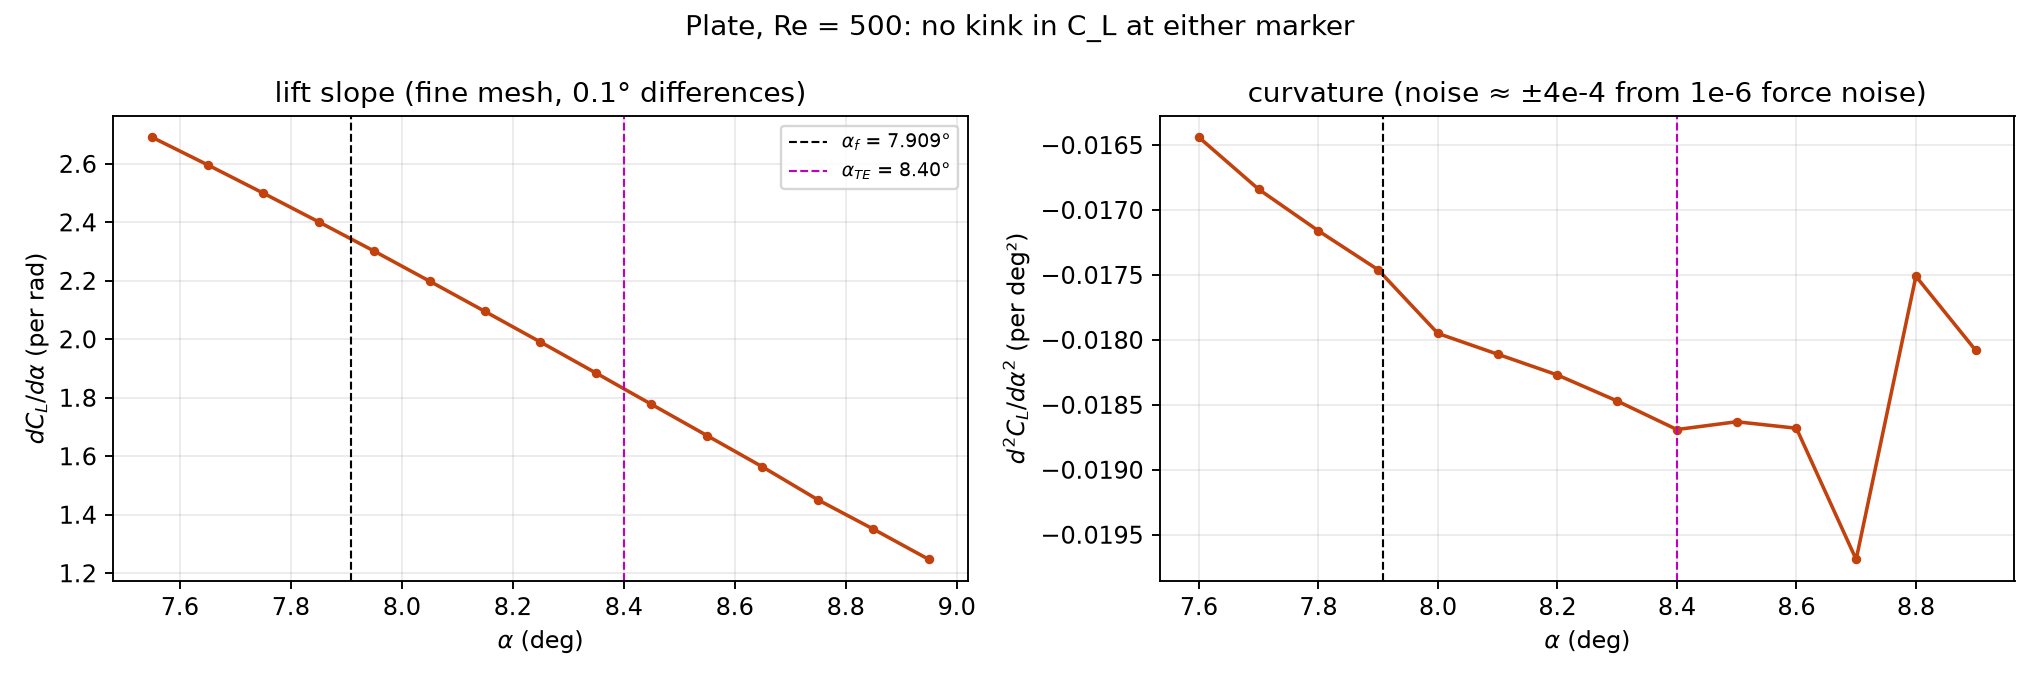
\includegraphics[width=\linewidth]{hypothesis/slope_curvature_markers.png}
\caption{Fine-mesh lift slope and curvature from $0.1^\circ$ differences. The slope is straight
through both markers. The curvature effects (about $5\times10^{-4}$) are at the noise level set
by $10^{-6}$ force convergence.}
\label{fig:kink}
\end{figure}

\FloatBarrier
\section{The bubble in pictures (fine mesh)}

The bubble forms at $\af = 7.909^\circ$ as a single point at $x = 0.225$. Just after formation its
length grows as $(\alpha-\af)^{0.53\text{--}0.61}$. It then grows mostly downstream until its
reattachment reaches the trailing edge at $\ate \approx 8.40^\circ$, after which it stays closed,
pinned at the trailing edge.

\begin{figure}[h]
\centering
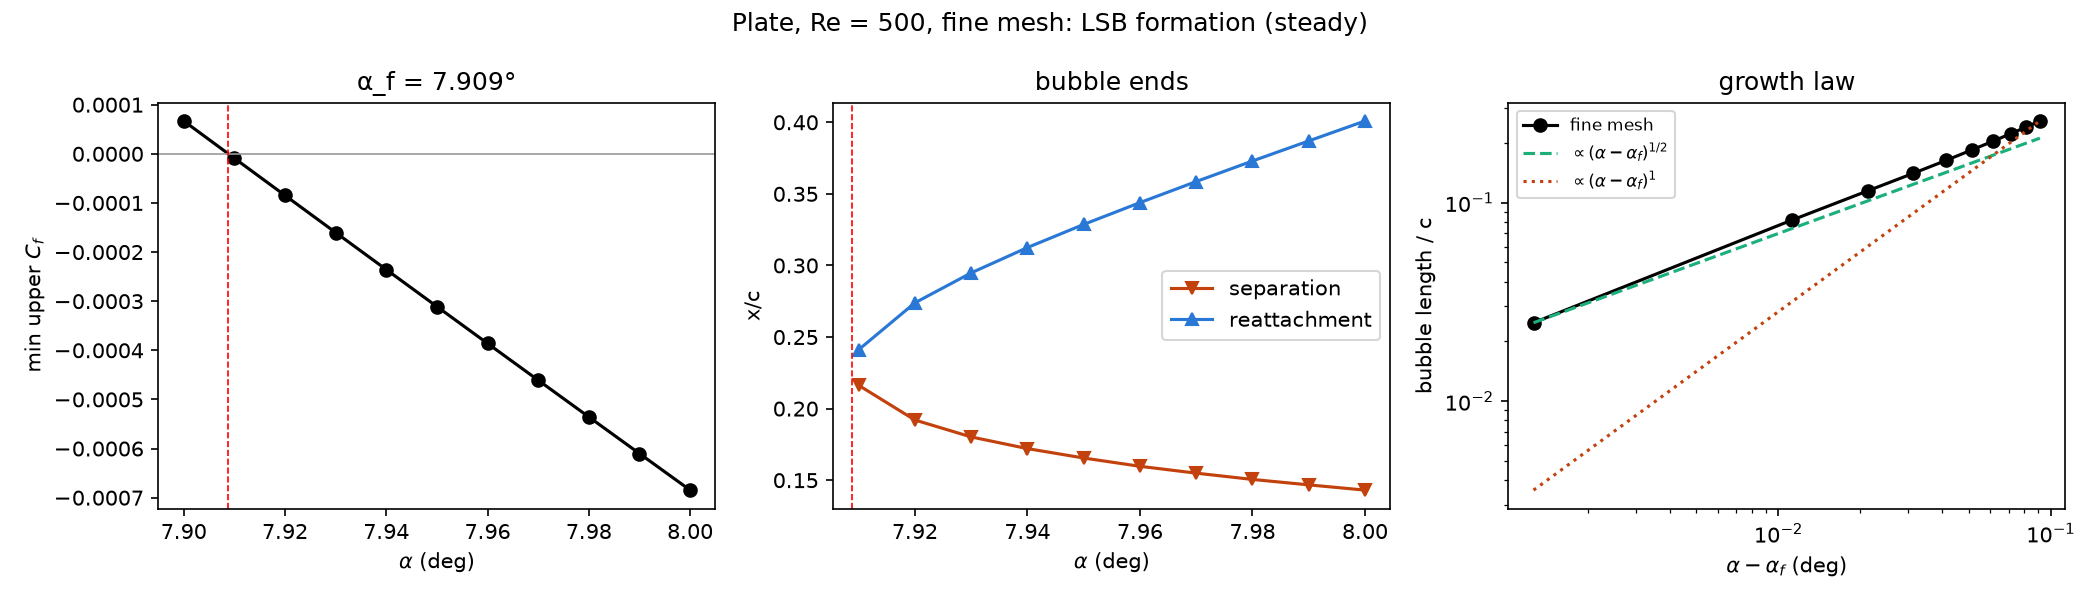
\includegraphics[width=\linewidth]{plate_fine/formation.png}
\caption{Formation. Left: $C_{f,\min}$, which is linear in $\alpha$. Centre: separation and
reattachment. Right: bubble length against $\alpha-\af$, close to $\propto(\alpha-\af)^{1/2}$.}
\end{figure}

\begin{figure}[h]
\centering
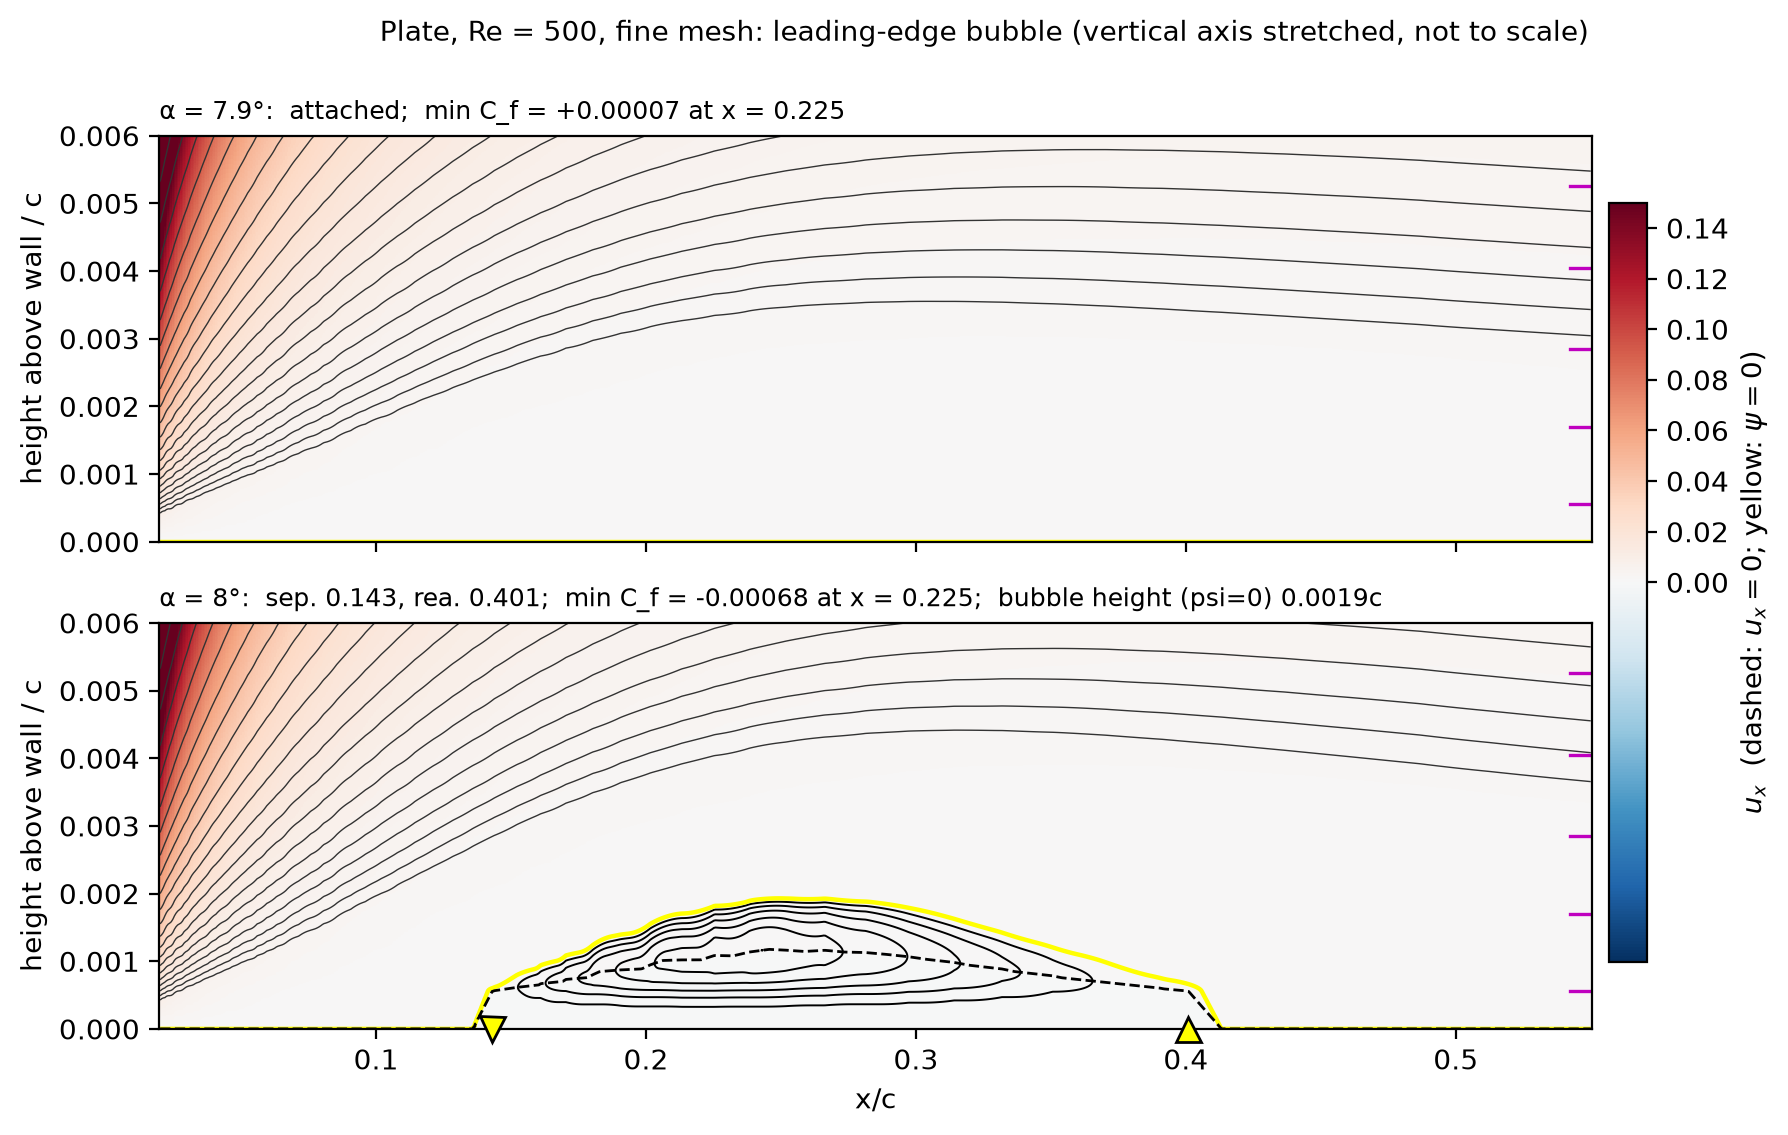
\includegraphics[width=\linewidth]{plate_fine/bubble_zoom_7.9_8.png}
\caption{$7.9^\circ$ (attached) and $8.0^\circ$ (bubble from 0.143 to 0.401). The vertical axis
is stretched. Yellow: the dividing streamline $\psi=0$. Dashed: $u_x=0$. Magenta ticks: cell
centres.}
\end{figure}

\begin{figure}[h]
\centering
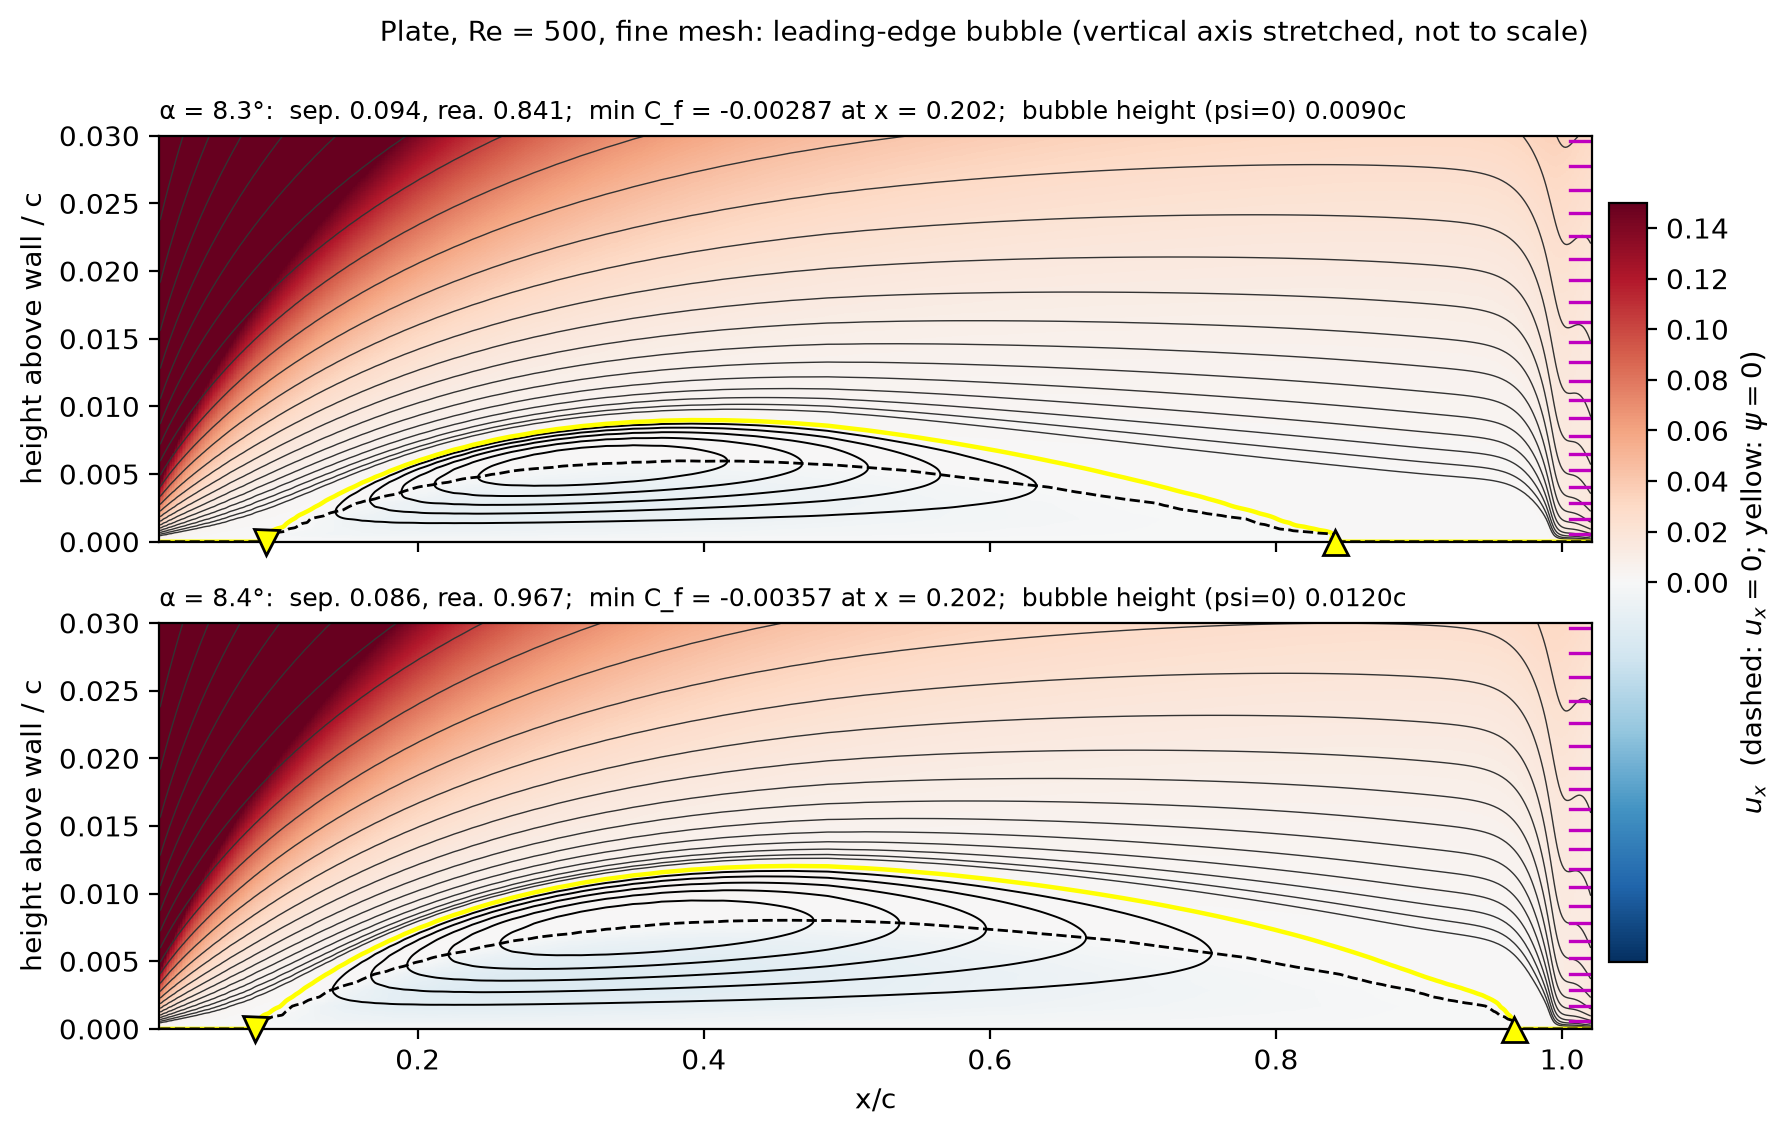
\includegraphics[width=\linewidth]{plate_fine/bubble_zoom_8.3_8.4.png}
\caption{$8.3^\circ$ (reattachment 0.841) and $8.4^\circ$ (0.967): the reattachment point reaches
the trailing edge. This is $\ate$ as defined in this report.}
\end{figure}

\begin{figure}[h]
\centering
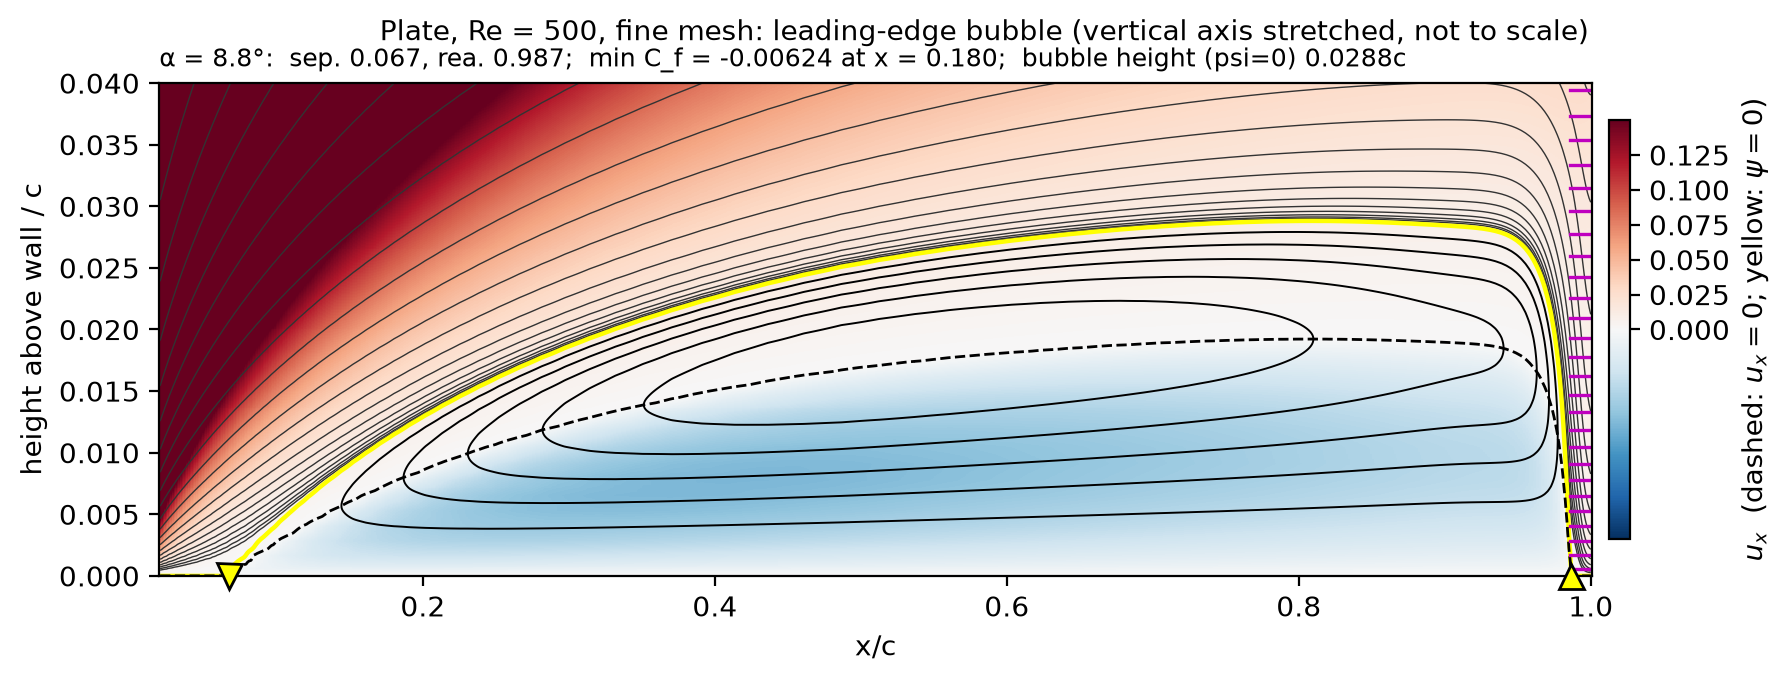
\includegraphics[width=\linewidth]{plate_fine/bubble_zoom_8.8.png}
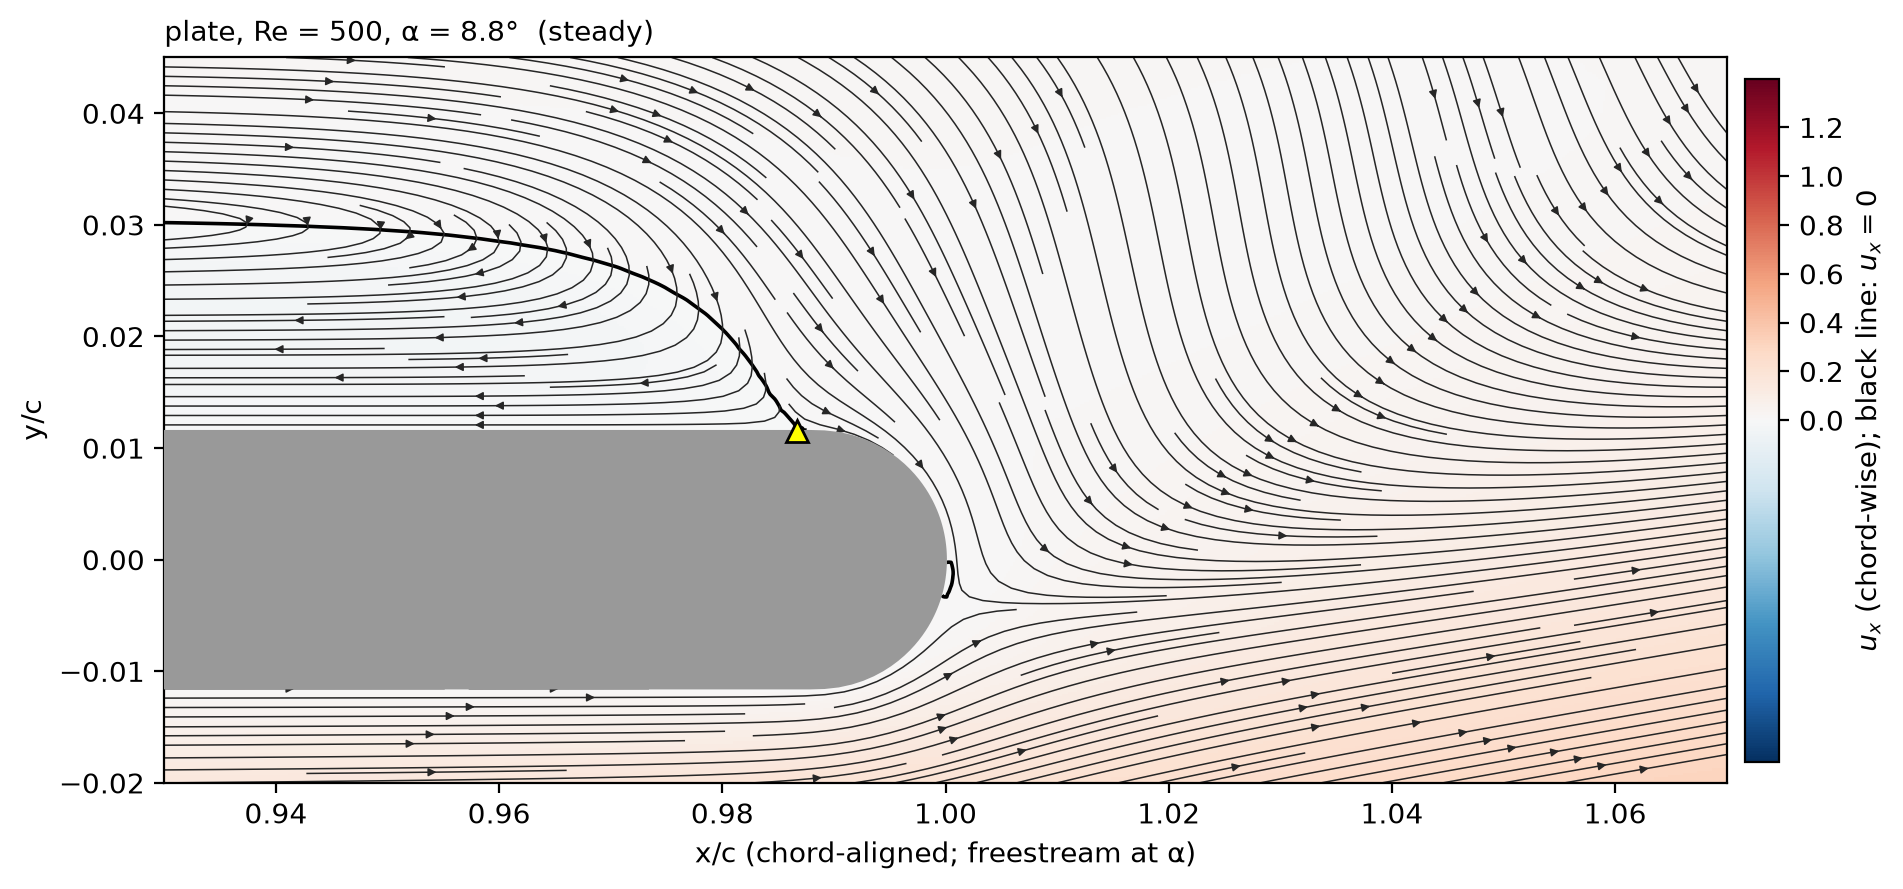
\includegraphics[width=0.8\linewidth]{plate_fine/aoa8.8/streamlines_te.png}
\caption{$8.8^\circ$. Top: the bubble covers the upper surface and stays closed. Bottom: the
trailing edge at true scale. Flow from the lower surface wraps around the rounded edge, and the
bubble's rear stagnation point sits at the corner (0.987). There is no recirculation in the
wake.}
\end{figure}

\FloatBarrier
\section{Caveats}
\begin{enumerate}[leftmargin=*]
\item \textbf{The meaning of $\ate$ was chosen, not observed} (see the box on page~1). Fits~(A)
  and~(B) depend on it.
\item \textbf{Bubble resolution.} At formation the reversed flow is a single cell row thick.
  $\af$ hardly depends on the mesh ($7.892^\circ$ against $7.909^\circ$), but bubble lengths
  near formation are uncertain at the 10\,\% level.
\item \textbf{Steady solutions above $11.33^\circ$.} The $8.5$--$12^\circ$ fit includes steady
  solutions of a flow that actually sheds. The $8.5$--$11.25^\circ$ row leaves them out.
\item \textbf{Only the plate is tested.} The hypothesis concerns a trend across sections. Note
  that the NACA0012 at Re = 500 has no leading-edge bubble, yet its two-term fit holds to
  $9^\circ$. That too points away from the bubble as the source of the cubic.
\end{enumerate}

\end{document}
